% !TeX root = ../main.tex

\chapter{案例分析}

本章為案例分析,第一部分進行風速預測分析,並計算不同預測模型的誤差結果來比較模型的預測能力,第二部分進行收益結果分析,並透過控制參數比較在不同情況下之收益結果。

\section{模擬情境概述}

% 設備概述
本研究模擬與分析所使用的電腦,其硬體設備採用 Intel® Core™ i7 處理器,記憶體共 24 GB,運行 Microsoft Windows 10 作業系統。並使用 MathWorks 公司出品的商業數學軟體 MATrix LABoratory (MATLAB) 與以程式語言 Python 為基礎的數值分析與統計模型套件進行模擬與分析之程式開發。

% 風力資料
關於歷史風速資料與模擬場址的選擇,考量我國\uline{澎湖}、\uline{金門}與\uline{馬祖}地區由於孤立於臺灣本島的電力傳輸系統之外,較適合作為含風力發電與電動汽車的的虛擬電廠參與電力市場交易的模擬案例。本文使用\uline{東吉島}(DONGJIDAO)測站(北緯 $23^\circ 15' 32''$,東經 $119^\circ 39'34''$)於 2018 年的風速資料,並根據表 \ref{table: Taiwan Wind Farm Data} 所示的我國風力發電場址資料,假設模型中的風力電場由八座 Enercon E40/600 Model 風力發電機組與四座 Enercon E44/900 Model 風力發電機組所構成。

% 電力價格
收益分析部分的電力價格將採用因應不同用電狀況與發電情況所制定的時間電價(Time of Use Price, TOU),這樣一來虛擬電廠在參與電力市場時,可以根據時間電價制定發電計畫,用以平衡波動並獲取較大收益,比如在離峰時段儲存電能至電動汽車,而在尖峰時段販售電力。但由於我國智慧電錶尚未完全普及,因此未能有效針對不同時段制定電價,而是以季節區分並制定大略峰值時段電價,本文將採用表 \ref{table: Electric Price} 所示的臺灣電力公司非夏季兩段式電價進行收益計算 \cite{taipower2018price}。

\begin{table}[htp]
  \centering
  \caption[臺灣電力公司非夏季兩段式電價]{臺灣電力公司非夏季的兩段式電價 \cite{taipower2018price}}
  \begin{tabular}{cr}
    \toprule
    \textbf{時間}   & \textbf{電價(元/度)}   \\
    \midrule
    00:00 - 07:30   & NT \$1.73                \\
    07:30 - 22:30   & NT \$4.23                \\
    22:30 - 24:00   & NT \$1.73                \\
    \bottomrule
  \end{tabular}
  \label{table: Electric Price}
\end{table}

% 電動汽車

\section{風速預測分析}

\subsection{歷史風速概述}

此處採用\uline{東吉島}(DONGJIDAO)測站於 $2018$ 年間風速跨度較大的十二月份歷史風速資料進行風力電場短期發電預測示範計算,取該月份中前二十九日共 $696$ 個小時的歷史風速作為觀測資料,預測最後二日共 $48$ 小時的短期風速,並比較不同預測模型的誤差結果。在後續內容中,將選擇預測能力較佳的模型進行全年預測以作為收益分析中參與虛擬電廠的風力電場發電數量。

圖 \ref{figure: Historial Wind Speed} 為根據\uline{東吉島}(DONGJIDAO)測站 $2018$ 年十二月份的歷史風速資料所繪製的原始風速時間序列,顯示在該月份中所測得之歷史風速有較大幅度的變化,且初步判斷該時間序列具備趨勢性故為非平穩時間序列。

\begin{figure}[htbp]
  \centering
  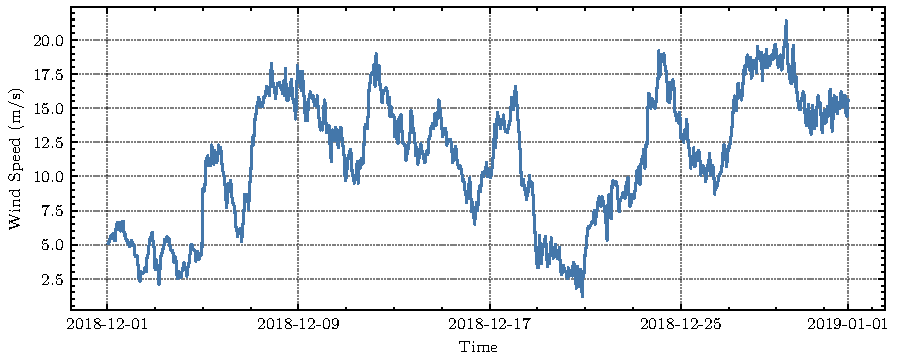
\includegraphics[width=\textwidth]{Historial Wind Speed}
  \caption{原始風速時間序列}
  \label{figure: Historial Wind Speed}
\end{figure}

由於採用圖形檢驗法觀察時間序列平穩性可能根據觀察者不同而存在主觀性差異,本文採用 Augmented Dickey-Fuller 檢定進行單根檢驗,其平穩性檢驗結果如表 \ref{table: Raw Time Series ADF Result} 所示,由於 ADF 檢驗統計量並不同時小於在 $99\%$、$95\%$ 與 $90\%$ 信賴區間下的 ADF 臨界檢驗值,因此原始風速資料時間序列為非平穩時間序列。

\begin{table}[htbp]
  \centering
  \caption[原始風速時間序列 ADF 檢定結果]{原始風速時間序列 ADF 檢定結果}
  \begin{tabular}{lr}
    \toprule
    \textbf{檢驗統計量} & \textbf{數值}     \\
    \midrule
    Test Statistic          & $-3.217446$   \\
    p-value                 & $1.8997 \times 10^{-2}$    \\
    Critical Value ($1\%$)  & $-3.439377$   \\
    Critical Value ($5\%$)  & $-2.865524$   \\
    Critical Value ($10\%$) & $-2.568891$   \\
    \bottomrule
  \end{tabular}
  \label{table: Raw Time Series ADF Result}
\end{table}

\subsection{單一預測模型}

\subsubsection{ARIMA 模型}

由於 ARIMA 模型的概念在於透過歷史資料的自相關性進行未來結果的預測,為使採用樣本時間序列所得到的擬合曲線在未來短期時間內延續既有型態,所採用的時間序列須具備平穩性。由前述內容已知原始風速時間序列為非平穩時間序列,因此需反覆計算時間序列中當前時刻與前一時刻的差值來取得其差分後的平穩時間序列。

\begin{figure}[htbp]
  \centering
  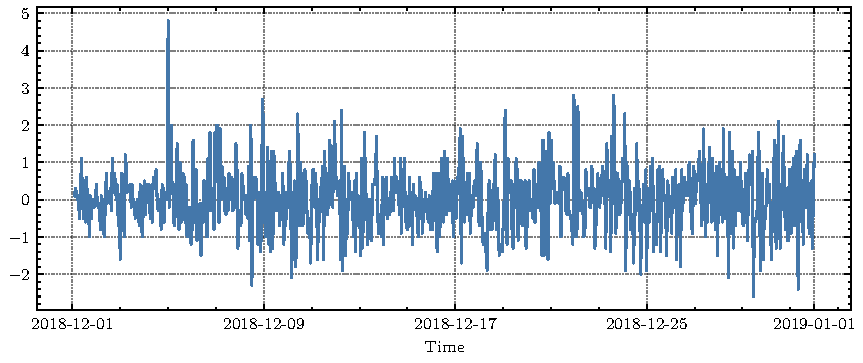
\includegraphics[width=\textwidth]{Difference Wind Speed}
  \caption{差分風速時間序列}
  \label{figure: Difference Wind Speed}
\end{figure}

將原始風速時間序列進行一階差分後所得到的差分風速時間序列如圖 \ref{figure: Difference Wind Speed} 所示,由圖形可初步判斷該時間序列已具備平穩性。為避免觀察者不同而存在的主觀性差異,採用 Augmented Dickey-Fuller 檢定進行單根檢驗的平穩性檢驗結果如表 \ref{table: Difference Time Series ADF Result} 所示,其中 ADF 檢驗統計量已同時小於在 $99\%$、$95\%$ 與 $90\%$ 信賴區間下的 ADF 臨界檢驗值,且 p-value 已十分接近零,因此該差分風速時間序列已為平穩時間序列。

\begin{table}[htbp]
  \centering
  \caption[差分風速時間序列 ADF 檢定結果]{差分風速時間序列 ADF 檢定結果}
  \begin{tabular}{lr}
    \toprule
    \textbf{檢驗統計量} & \textbf{數值}     \\
    \midrule
    Test Statistic          & $-21.391265$  \\
    p-value                 & $5.817483 \times 10^{-27}$    \\
    Critical Value ($1\%$)  & $-3.439206$   \\
    Critical Value ($5\%$)  & $-2.865448$   \\
    Critical Value ($10\%$) & $-2.568851$   \\
    \bottomrule
  \end{tabular}
  \label{table: Difference Time Series ADF Result}
\end{table}

圖 \ref{figure: Difference Wind Speed ACF}  和圖 \ref{figure: Difference Wind Speed PACF} 分別為差分時間序列的自相關係數函數(Autocorrelation Function, ACF)圖與非自相關係數函數(Partial Autocorrelation Function, PACF)圖,由圖形可知其自相關係數函數在延遲項 Lag 值為 $2$ 時落入信賴區間中,其偏自相關係數函數在延遲項 Lag 值為 $3$ 時落入信賴區間中,據此可認定其時間序列具備平穩性並可大致識別其模型可採用 $\text{ARIMA} (2, 1, 3)$。

\begin{figure}[htbp]
  \centering
  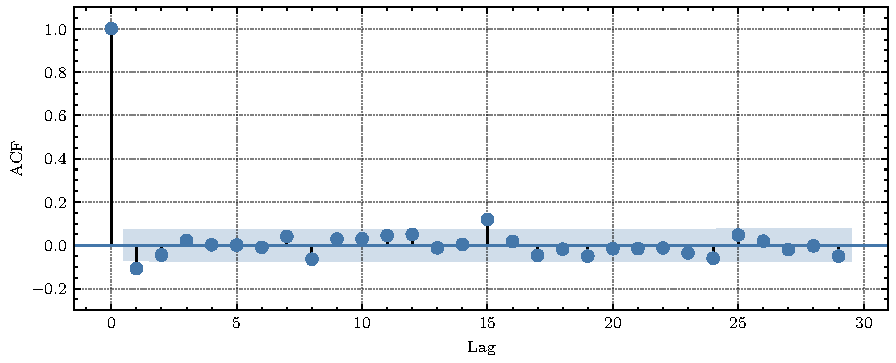
\includegraphics[width=\textwidth]{Difference Wind Speed ACF}
  \caption{差分時間序列自相關係數函數(ACF)圖}
  \label{figure: Difference Wind Speed ACF}
\end{figure}

\begin{figure}[htbp]
  \centering
  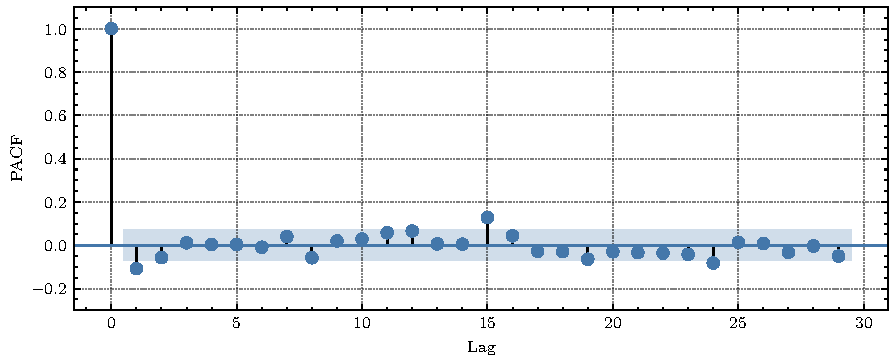
\includegraphics[width=\textwidth]{Difference Wind Speed PACF}
  \caption{差分時間序列偏自相關係數函數(PACF)圖}
  \label{figure: Difference Wind Speed PACF}
\end{figure}

透過自相關係數函數圖與偏自相關係數函數圖進行模型定階可能存在主觀性差異,通常會使用 AIC(Akaike's Information Criterion)及 BIC(Bayesian Information Criterion)作為評價模型優劣的指標,採用窮舉法擬合所有模型並選出具有較小 AIC 值的最適模型。表 \ref{table: Auto ARIMA Result} 為使用開放式源代碼套件 \texttt{pyramid} 所提供的 \texttt{auto\_arima()} 函數針對差分時間序列模型進行窮舉擬合所得到的結果,採用 AIC 值最小的 $\text{ARIMA} (2, 1, 0)$ 模型進行短期預測,預測結果如圖 \ref{figure: Wind Speed Prediction ARIMA} 所示。

\begin{table}[htbp]
  \centering
  \caption[差分風速時間序列 $\text{ARIMA}(p, d, q)$ 適配檢驗]{差分風速時間序列 $\text{ARIMA}(p, d, q)$ 適配檢驗}
  \begin{tabular}{cccc}
    \toprule
    \textbf{模型} & \textbf{AIC} & \textbf{BIC} & \textbf{Time} \\
    \midrule
    $\text{ARIMA}(1,1,1)$ & $1886.365$ & $1904.808$ & $0.229$ \si{s} \\
    $\text{ARIMA}(1,1,2)$ & $1886.528$ & $1909.581$ & $0.424$ \si{s} \\
    $\text{ARIMA}(1,1,3)$ & $1888.300$ & $1915.964$ & $0.404$ \si{s} \\
    $\text{ARIMA}(1,1,4)$ & $1890.242$ & $1922.517$ & $0.619$ \si{s} \\
    $\text{ARIMA}(2,1,0)$ & $1885.681$ & $1904.124$ & $0.087$ \si{s} \\
    $\text{ARIMA}(2,1,1)$ & $1887.588$ & $1910.641$ & $0.258$ \si{s} \\
    $\text{ARIMA}(2,1,2)$ & $1889.564$ & $1917.228$ & $0.165$ \si{s} \\
    $\text{ARIMA}(2,1,3)$ & $1890.281$ & $1922.556$ & $0.890$ \si{s} \\
    $\text{ARIMA}(3,1,0)$ & $1887.576$ & $1910.630$ & $0.110$ \si{s} \\
    $\text{ARIMA}(3,1,1)$ & $1889.572$ & $1917.236$ & $0.155$ \si{s} \\
    $\text{ARIMA}(3,1,2)$ & $1890.944$ & $1923.219$ & $0.955$ \si{s} \\
    $\text{ARIMA}(4,1,0)$ & $1889.565$ & $1917.229$ & $0.138$ \si{s} \\
    $\text{ARIMA}(4,1,1)$ & $1891.564$ & $1923.839$ & $0.184$ \si{s} \\
    \bottomrule
  \end{tabular}
  \label{table: Auto ARIMA Result}
\end{table}

\begin{figure}[htbp]
  \centering
  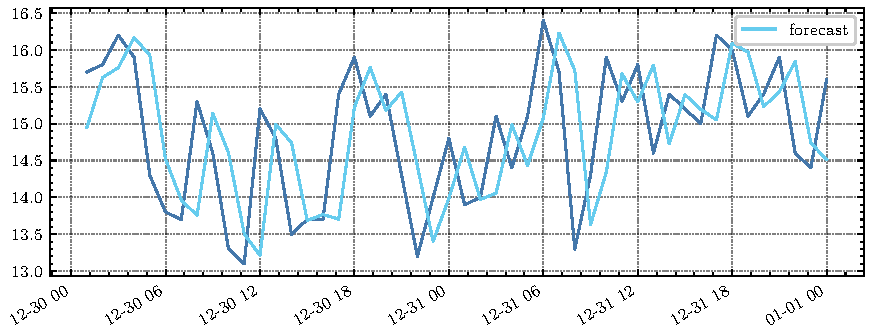
\includegraphics[width=\textwidth]{Wind Speed Prediction (ARIMA)}
  \caption{單一 ARIMA 模型短期風速預測結果}
  \label{figure: Wind Speed Prediction ARIMA}
\end{figure}

\subsubsection{SVR 模型}

基於支持向量迴歸模型進行時間序列預測時,在將歷史風速資料進行標準化後,採用時間間隔為 $1$ 單位的延遲,並選用高斯徑向核函數進行預測。使用開放式源代碼套件 \texttt{sklearn} 所提供的 \texttt{SVR()} 函數針對風速時間序列模型進行預測的結果如圖 \ref{figure: Wind Speed Prediction SVR} 所示。

\begin{figure}[htbp]
  \centering
  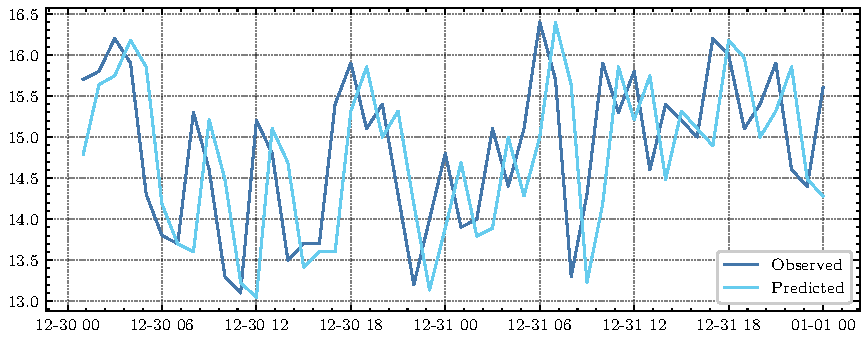
\includegraphics[width=\textwidth]{Wind Speed Prediction (SVR)}
  \caption{單一 SVR 模型短期風速預測結果}
  \label{figure: Wind Speed Prediction SVR}
\end{figure}

\subsection{組合預測模型}

\subsubsection{一般等權 ARIMA-SVR 組合模型}

本文採用的一般等權 ARIMA-SVR 組合模型如方程式 \eqref{equation: Normal Combine Model} 所示,即使用相等權重將前述單一預測模型中 ARIMA 模型與 SVR 模型的預測結果進行線性組合。根據單一 ARIMA 模型與單一 SVR 模型預測結果進行相等權重線性組合的預測結果如圖 \ref{figure: Wind Speed Prediction Linear} 所示。

\begin{figure}[htbp]
  \centering
  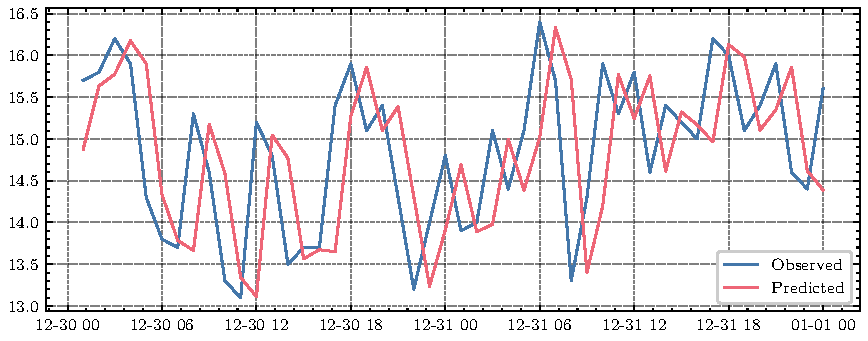
\includegraphics[width=\textwidth]{Wind Speed Prediction (Linear)}
  \caption{一般等權 ARIMA-SVR 組合模型短期風速預測結果}
  \label{figure: Wind Speed Prediction Linear}
\end{figure}

\subsubsection{小波分解 ARIMA-SVR 組合模型}

本文採用的小波分解 ARIMA-SVR 組合模型如方程式 \eqref{equation: Wavelet Combine Model} 所示,即將時間序列透過離散小波轉換分解為高頻部分(細節分量)與低頻部分(近似分量),並分別採用 ARIMA 模型預測與 SVR 模型預測,再將預測結果進行重構與整合。

針對時間序列採用較平滑且解析度較高的 Daubechies Wavelet 小波或 Symlet 小波進行分解較為合適。本文使用不同消失矩 $N$ 的 Daubechies Wavelet 小波將原始風速時間序列進行不同 層數的訊號分解後進行訊號重構所得到的誤差如表 \ref{table: Wavelet Reconstruction Error} 所示,顯示採用 db4 小波進行 $2$ 層的訊號分解能夠在訊號重構時產生較小的誤差。

\begin{table}[htp]
  \centering
  \caption[原始風速時間序列進行小波分解的重構誤差]{原始風速時間序列進行小波分解的重構誤差}
  \begin{tabular*}{0.65\textwidth}{lcccc}
    \toprule
    \textbf{分解層數} & $\text{db}_3$ \textbf{小波} & $\text{db}_4$ \textbf{小波} & $\text{db}_5$ \textbf{小波} & $\text{db}_6$ \textbf{小波} \\
    \midrule
    $2$ 層分解 & $2.8931$ & $1.1759$ & $4.2143$ & $3.2171$ \\
    $3$ 層分解 & $4.1932$ & $2.1486$ & $5.9631$ & $4.7622$ \\
    $4$ 層分解 & $4.3194$ & $3.0123$ & $7.3174$ & $5.4318$ \\
    \bottomrule
    & & & & ($\times 10^{-10}$)
  \end{tabular*}
  \label{table: Wavelet Reconstruction Error}
\end{table}

在使用開放式源代碼套件 \texttt{pywt} 所提供的 \texttt{wavedec()} 函數,選擇 db4 小波對原始風速時間序列進行 $2$ 層小波分解與重構後,可以得到如圖 \ref{figure: Approximated Component Level 2 (A2)} 所示反映整體趨勢的近似分量 $A1$,以及如圖 \ref{figure: Detailed Component Level 2 (D2)} 和圖 \ref{figure: Detailed Component Level 1 (D1)} 所示反映細小波動的細節分量 $D2$ 和 $D1$。

\begin{figure}[hbp]
  \centering
  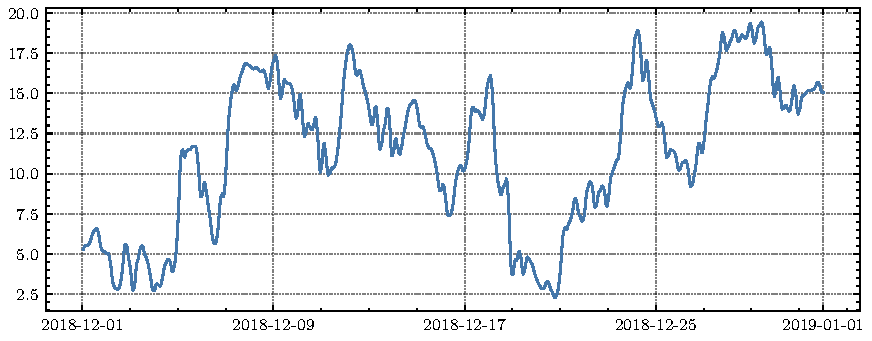
\includegraphics[width=\textwidth]{Approximated Component in Level 2 (A2)}
  \caption{原始風速時間序列進行小波分解的近似分量 $A2$}
  \label{figure: Approximated Component Level 2 (A2)}
  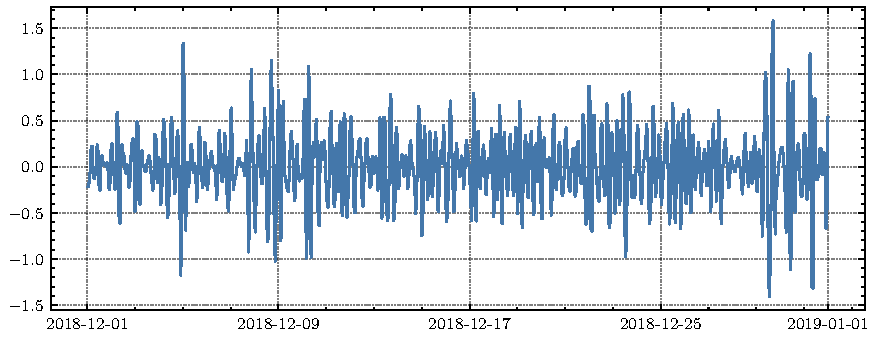
\includegraphics[width=\textwidth]{Detailed Component in Level 2 (D2)}
  \caption{原始風速時間序列進行小波分解的細節分量 $D2$}
  \label{figure: Detailed Component Level 2 (D2)}
  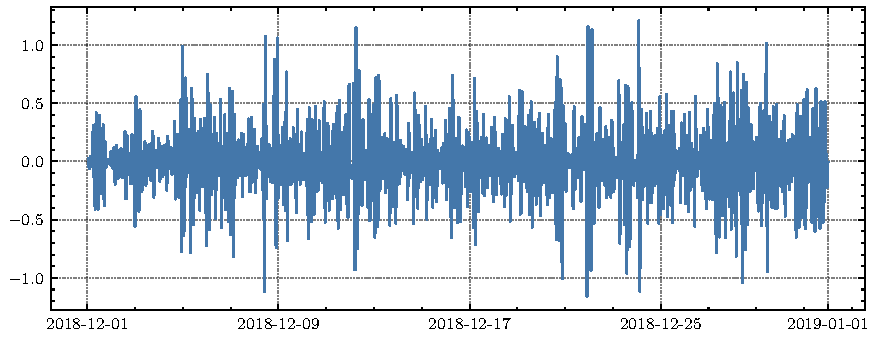
\includegraphics[width=\textwidth]{Detailed Component in Level 1 (D1)}
  \caption{原始風速時間序列進行小波分解的細節分量 $D1$}
  \label{figure: Detailed Component Level 1 (D1)}
\end{figure}

採用 Augmented Dickey-Fuller 檢定對原始風速時間序列經小波分解後所得到的細節分量 $D2$ 和 $D1$ 進行單根檢驗,其平穩性檢驗結果分別如表 \ref{table: D2 ADF Result} 和表 \ref{table: D1 ADF Result} 所示,其中 ADF 檢驗統計量皆已同時小於在 $99\%$、$95\%$ 與 $90\%$ 信賴區間下的 ADF 臨界檢驗值,且 p-value 已十分接近零,因此細節分量 $D2$ 和 $D1$ 皆為平穩時間序列。

\begin{table}[htbp]
  \centering
  \caption[原始風速時間序列 $D2$ 細節分量 ADF 檢定結果]{原始風速時間序列 $D2$ 細節分量 ADF 檢定結果}
  \begin{tabular}{lr}
    \toprule
    \textbf{檢驗統計量} & \textbf{數值}     \\
    \midrule
    Test Statistic          & $-13.40788$  \\
    p-value                 & $4.433267 \times 10^{-25}$    \\
    Critical Value ($1\%$)  & $-3.439427$   \\
    Critical Value ($5\%$)  & $-2.865446$   \\
    Critical Value ($10\%$) & $-2.568903$   \\
    \bottomrule
  \end{tabular}
  \label{table: D2 ADF Result}
\end{table}

\begin{table}[htbp]
  \centering
  \caption[原始風速時間序列 $D1$ 細節分量 ADF 檢定結果]{原始風速時間序列 $D1$ 細節分量 ADF 檢定結果}
  \begin{tabular}{lr}
    \toprule
    \textbf{檢驗統計量} & \textbf{數值}     \\
    \midrule
    Test Statistic          & $-15.85389$  \\
    p-value                 & $9.380079 \times 10^{-29}$    \\
    Critical Value ($1\%$)  & $-3.439427$   \\
    Critical Value ($5\%$)  & $-2.865446$   \\
    Critical Value ($10\%$) & $-2.568903$   \\
    \bottomrule
  \end{tabular}
  \label{table: D1 ADF Result}
\end{table}

如同前述步驟,針對細節分量 $D2$ 與 $D1$ 進行窮舉擬合後,分別選用 $\text{ARIMA} (2, 0, 2)$ 與 $\text{ARIMA} (2, 0, 1)$ 模型進行預測,並對近似分量 $A1$ 採用向量迴歸模型進行預測。最後將兩者預測結果進行整合可得到小波分解 ARIMA-SVR 組合模型的短期風速預測結果如圖 \ref{figure: Wind Speed Prediction Wavelet} 所示。

\begin{figure}[htbp]
  \centering
  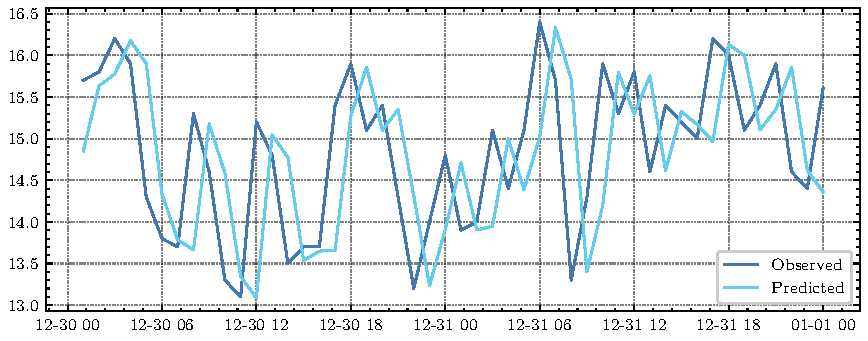
\includegraphics[width=\textwidth]{Wind Speed Prediction (Wavelet)}
  \caption{小波分解 ARIMA-SVR 組合模型短期風速預測結果}
  \label{figure: Wind Speed Prediction Wavelet}
\end{figure}

\subsection{模型誤差比較}

為比較在短期風速預測中採用小波分解 ARIMA-SVR 組合模型是否相較傳統單一預測模型具有較好的效果,本文中使用同一段時間內的歷史風速資料,分別採用了單一 ARIMA 預測模型、單一 SVR 預測模型、一般等權 ARIMA-SVR 組合模型與小波分解 ARIMA-SVR 組合模型進行預測。

計算其平均絕對百分比誤差(MAPE)、平均絕對誤差(MAE)與均方根誤差(RMSE)作為模型優劣的評價依據,結果如表 \ref{table: Time Series Model Result} 所示。

\begin{table}[htp]
  \centering
  \caption[風速預測模型評估結果]{風速預測模型評估結果}
  \begin{tabular}{lccc}
    \toprule
    \textbf{模型}               & \textbf{MAPE} & \textbf{MAE} & \textbf{RMSE} \\
    \midrule
    單一 ARIMA 預測模型         & $5.3022 \%$   & $0.7817$     & $0.9692$      \\
    單一 SVR 預測模型           & $5.4723 \%$   & $0.8113$     & $0.9869$      \\
    一般等權 ARIMA-SVR 組合模型 & $5.2852 \%$   & $0.7762$     & $0.9651$      \\
    小波分解 ARIMA-SVR 組合模型 & $5.1487 \%$   & $0.7319$     & $0.9517$      \\
    \bottomrule
  \end{tabular}
  \label{table: Time Series Model Result}
\end{table}

\section{收益結果分析}

\subsection{電動汽車有無影響}

比較同一風力電場在有電動汽車作為儲能設備參與虛擬電廠與沒有電動汽車作為儲能設備參與虛擬電廠的收益,使用模型預測控制方法進行求解。

將每個月份中,將整合了電動汽車作為儲能設備的虛擬電廠收益記為 $\text{Profit}_{\text{with EV}}(t)$,而未整合電動汽車作為儲能設備的虛擬電廠收益記為 $\text{Profit}_{\text{without EV}}(t)$,
則可以將整合了電動汽車作為儲能設備的虛擬電廠收益增長率表示如方程式 \eqref{equation: Profit Growth Rate} 所示。

\begin{equation}\label{equation: Profit Growth Rate}
  R_{\text{growth}} = \frac{\text{Profit}_{\text{with EV}}(t) - \text{Profit}_{\text{without EV}}(t)}{\text{Profit}_{\text{without EV}}(t)} \times 100 \%
\end{equation}

模擬結果顯示,整合了電動汽車作為儲能設備的虛擬電廠相較未整合電動汽車作為儲能設備的虛擬電廠,具有較高的收益。此外,當 $\sigma$ 值較小時,由於儲能成本較低,而使虛擬電廠在電力市場電價較低時,儘可能儲存電力並於電力市場電價較高時進行販售。

\subsection{電動汽車數量需求}

\section{小結}